\documentclass[dvipdfmx]{standalone}
\usepackage{tikz}

\begin{document}

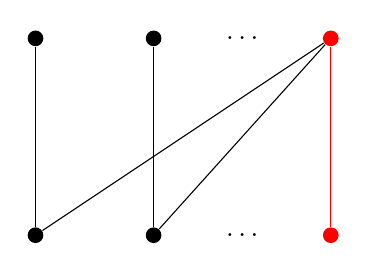
\begin{tikzpicture}
    \def\h{2.5}
    \def\w{1.5}
    \def\sep{1.5}
    \tikzset{dot/.style={circle, fill=black, inner sep=2pt}}
    \node[dot] (u1) at (0, \h) {};
    \node[dot] (u2) at (\w, \h) {};
    \node at (\w + \w*\sep*0.5, \h) {$\dots$};
    \node[dot, fill=red] (un) at (\w + \w*\sep, \h) {};
    
    \node[dot] (v1) at (0, 0) {};
    \node[dot] (v2) at (\w, 0) {}; 
    \node at (\w + \w*\sep*0.5, 0) {$\dots$};
    \node[dot, fill=red] (vn) at (\w + \w*\sep, 0) {};

    \draw (u1) -- (v1);
    
    \foreach \v in {v2} {
        \draw (u2) -- (\v);
    }
    \foreach \v in {v1, v2} {
        \draw (un) -- (\v);
    }
    \draw[red] (un) -- (vn);

\end{tikzpicture}

\end{document}